\documentclass[aspectratio=169]{beamer}

\usepackage{natbib}

\hypersetup{
    pdfauthor={Vineet John}, 
    colorlinks=true,
    linkcolor=black,
    citecolor=red,
    filecolor=magenta,
    urlcolor=cyan
}

\newcommand{\imgsrc}[1]{\tiny{Source: #1}}

\usetheme{metropolis}
\title{
	Disentangled Representation Learning\\
	for Linguistic Style Transfer}
\date{}
\author{Vineet John}
\institute{University of Waterloo}

\begin{document}

\maketitle

\graphicspath{{images/}}

\section{Motivation}

\begin{frame}{Universal Function Approximators}
	\centering
	\begin{figure}[ht]
		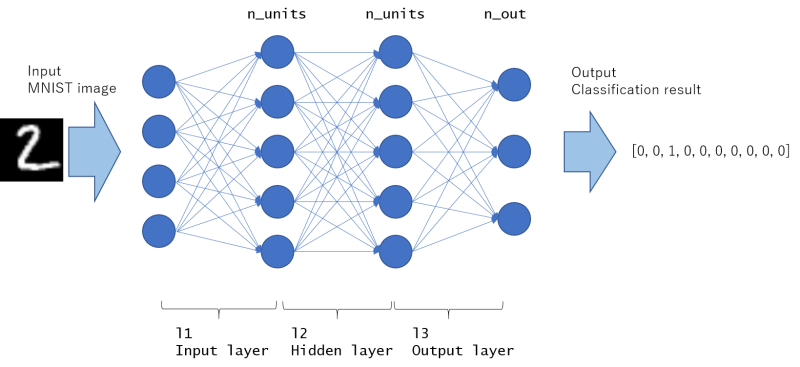
\includegraphics[width=\linewidth]{mlp-network}
	\end{figure}

    \imgsrc{\url{http://corochann.com/mnist-training-with-multi-layer-perceptron-1149.html}}
\end{frame}

\begin{frame}{Non-Interpretable Latent Representations}
	\begin{itemize}
		\item Neural networks can model arbitrarily complex functions
        \item The initial set of parameters are set randomly
        \item The learned parameters usually do not demonstrate a visible pattern.
	\end{itemize}

    \centering
    \begin{figure}[ht]
		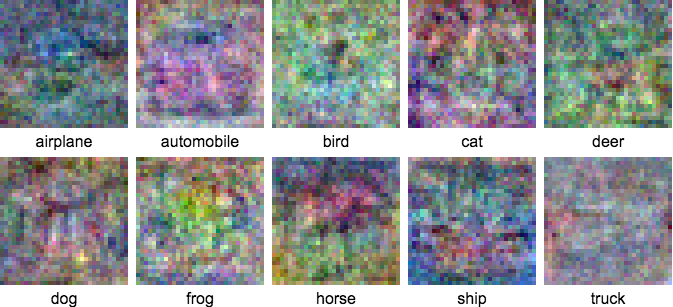
\includegraphics[width=0.6\linewidth]{uninterpretable-weights}
	\end{figure}
    
    \imgsrc{\url{https://ml4a.github.io/ml4a/looking_inside_neural_nets/}}
\end{frame}

\begin{frame}{Problem Statement}
	\centering
	\Huge{Generate plausible sentences in a user-defined style, while retaining the original content of the source sentences.}
\end{frame}

% 

\section{Background}

\begin{frame}{Autoencoding}
	\centering
	\begin{figure}[ht]
		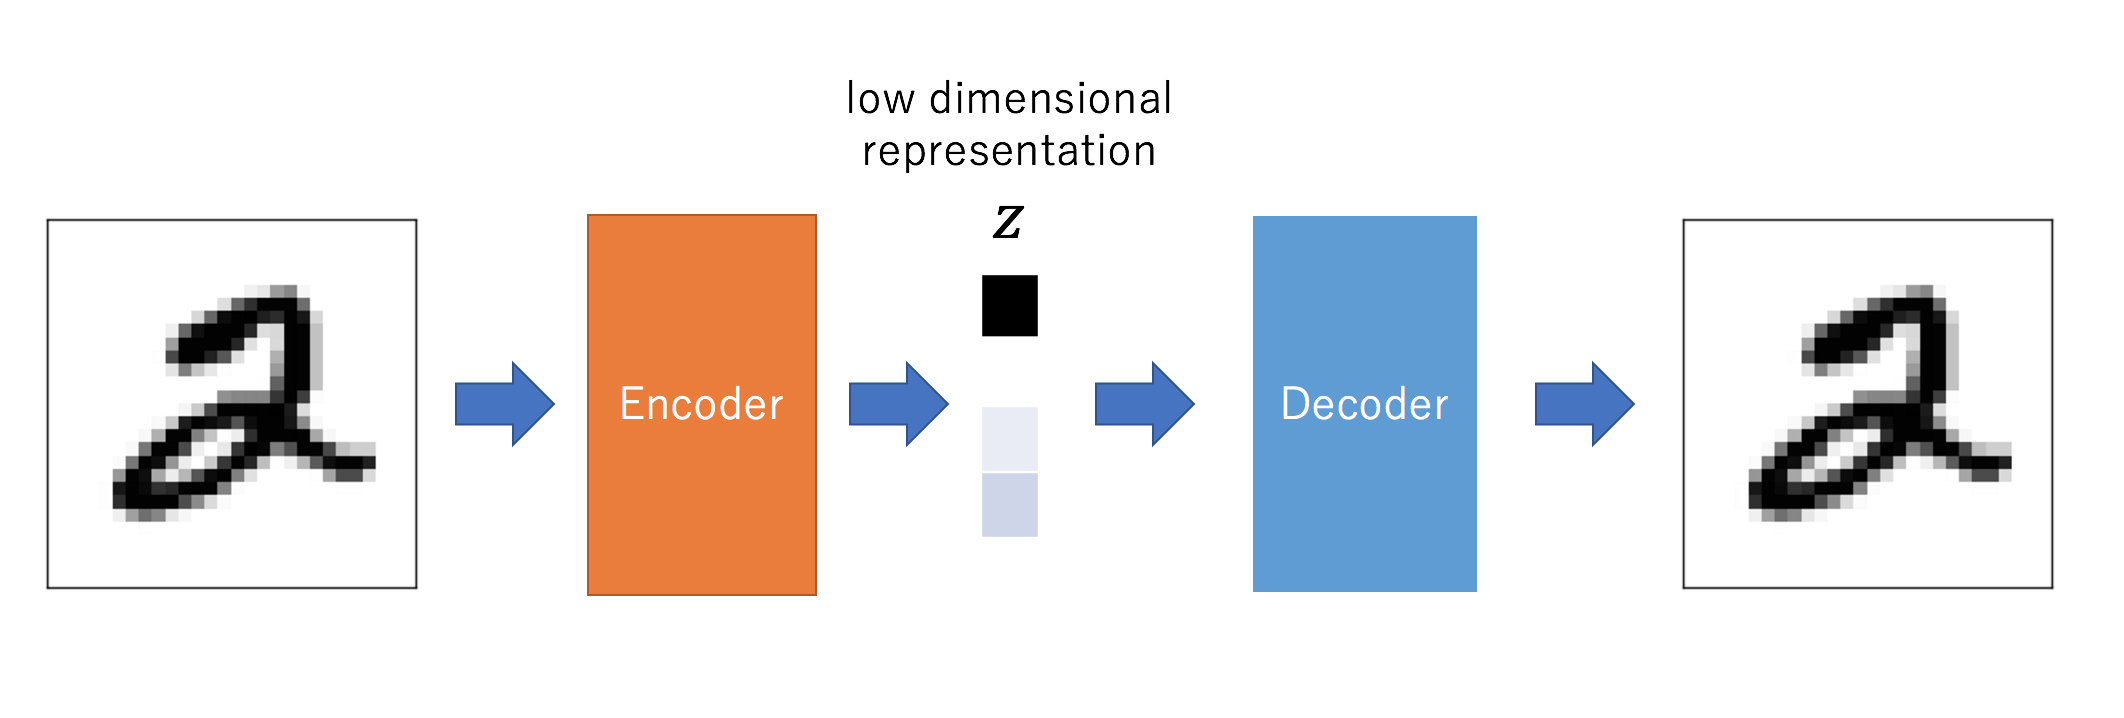
\includegraphics[width=\linewidth]{dae-structure}
	\end{figure}
    
    \imgsrc{\url{http://mlexplained.com/2017/12/28/an-intuitive-explanation-of-variational-autoencoders-vaes-part-1}}
\end{frame}

\begin{frame}{Variational Autoencoding}
	\centering
	\begin{figure}[ht]
		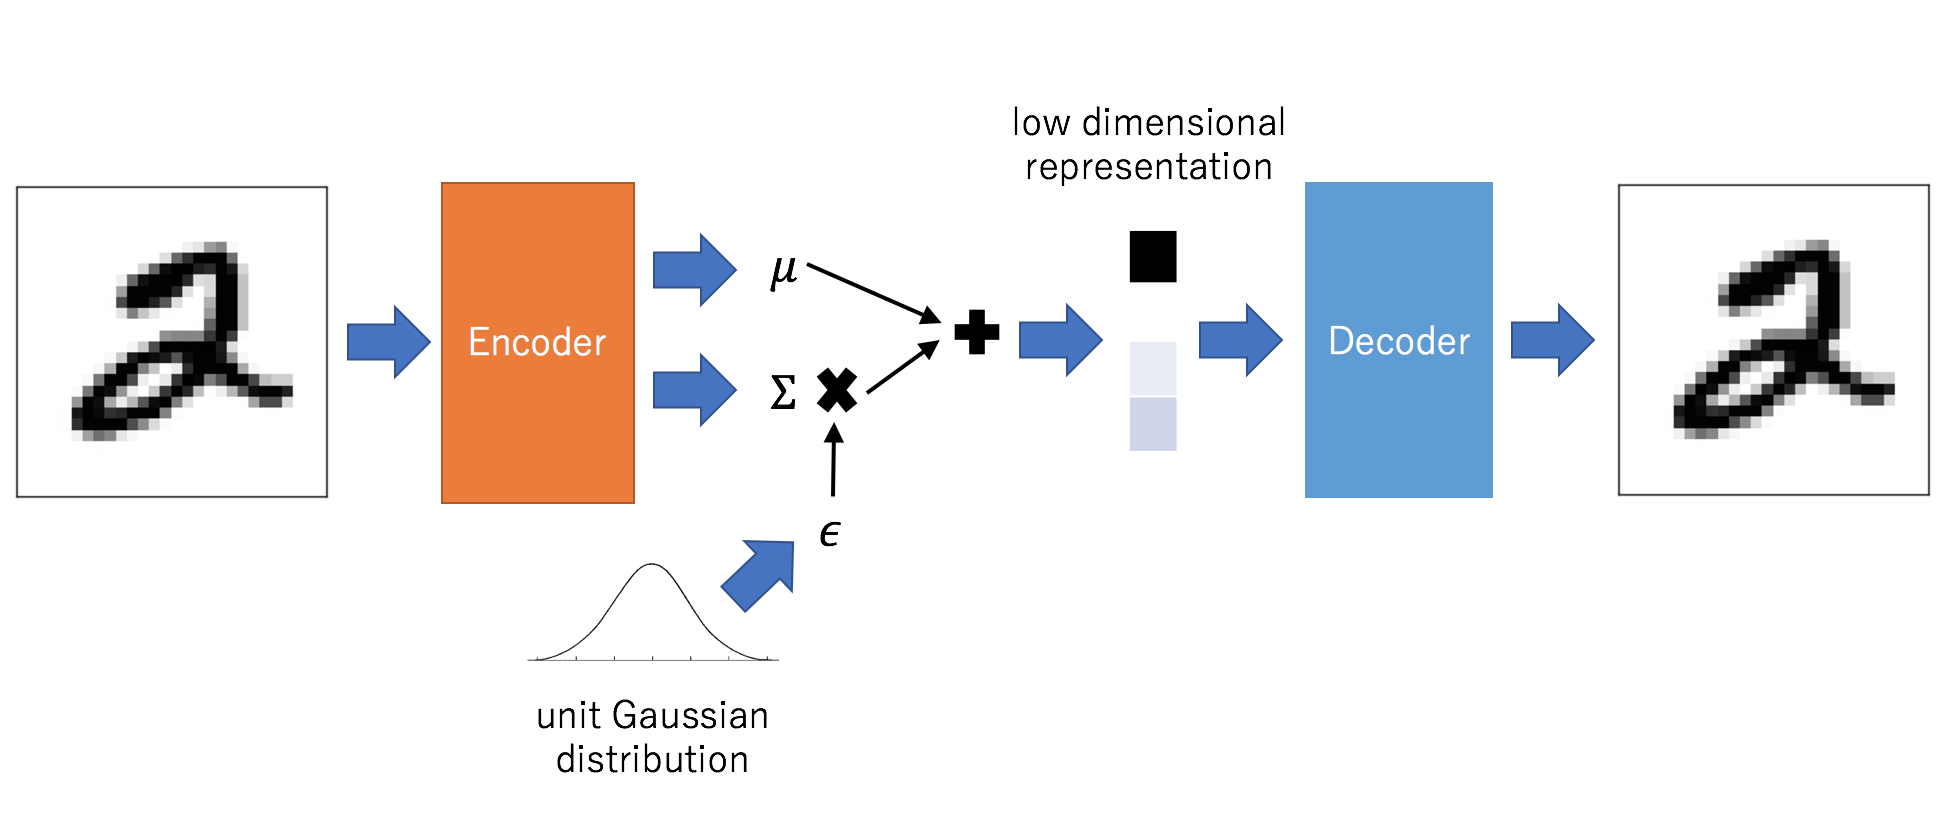
\includegraphics[width=\linewidth]{vae-structure}
	\end{figure}

    \imgsrc{\url{http://mlexplained.com/2017/12/28/an-intuitive-explanation-of-variational-autoencoders-vaes-part-1}}
\end{frame}

\begin{frame}{Sequence Autoencoding}
	\centering
	\makeatletter
\ifx\du\undefined
  \newlength{\du}
\fi
\setlength{\du}{\unitlength}
\ifx\spacing\undefined
  \newlength{\spacing}
\fi
\setlength{\spacing}{60\unitlength}
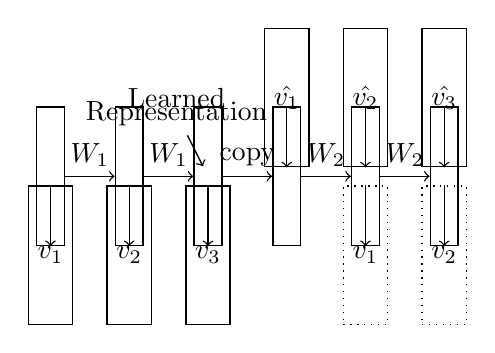
\begin{tikzpicture}
\pgfsetlinewidth{0.5\du}
\pgfsetmiterjoin
\pgfsetbuttcap

\node[rectangle, draw=black, minimum width=10\du, minimum height=50\du] (v1) at (0\spacing, 0) {$v_1$};
\node[rectangle, draw=black, minimum width=10\du, minimum height=50\du] (v2) at (\spacing, 0) {$v_2$};
\node[rectangle, draw=black, minimum width=10\du, minimum height=50\du] (v3) at (2\spacing, 0) {$v_3$};

\node[rectangle, dotted, draw=black, minimum width=10\du, minimum height=50\du] (v5) at (4\spacing, 0) {$v_1$};
\node[rectangle, dotted, draw=black, minimum width=10\du, minimum height=50\du] (v6) at (5\spacing, 0) {$v_2$};

\node[rectangle, draw=black, minimum width=10\du, minimum height=50\du] (h1) at (0\spacing, \spacing) {};
\node[rectangle, draw=black, minimum width=10\du, minimum height=50\du] (h2) at (\spacing, \spacing) {};
\node[rectangle, draw=black, minimum width=10\du, minimum height=50\du] (h3) at (2\spacing, \spacing) {};

\node[rectangle, draw=black, minimum width=10\du, minimum height=50\du] (h4) at (3\spacing, \spacing) {};
\node[rectangle, draw=black, minimum width=10\du, minimum height=50\du] (h5) at (4\spacing, \spacing) {};
\node[rectangle, draw=black, minimum width=10\du, minimum height=50\du] (h6) at (5\spacing, \spacing) {};

\node[rectangle, draw=black, minimum width=10\du, minimum height=50\du] (v4r) at (3\spacing, 2\spacing) {$\hat{v_1}$};
\node[rectangle, draw=black, minimum width=10\du, minimum height=50\du] (v5r) at (4\spacing, 2\spacing) {$\hat{v_2}$};
\node[rectangle, draw=black, minimum width=10\du, minimum height=50\du] (v6r) at (5\spacing, 2\spacing) {$\hat{v_3}$};

\node[anchor=center]  at (1.6\spacing, 2\spacing) {Learned};
\node[anchor=center] (p1) at (1.6\spacing, 1.8\spacing) {Representation};
\node[anchor=center] (p2) at (2\spacing, \spacing) {};
%\node[anchor=center] (w) at (0\spacing, 0.5\spacing) {$\WW_1$};

%\draw[ultra thick, ->] (2aa) -- node[left] {Conv Net} (3a);
\draw[->] (v1) -- (h1);
\draw[->] (v2) -- (h2);
\draw[->] (v3) -- (h3);
\draw[->] (v5) -- (h5);
\draw[->] (v6) -- (h6);

\draw[->] (h1) -- node[above] {$W_1$} (h2);
\draw[->] (h2) -- node[above] {$W_1$} (h3);
\draw[->] (h3) -- node[above] {copy} (h4);
\draw[->] (h4) -- node[above] {$W_2$} (h5);
\draw[->] (h5) -- node[above] {$W_2$} (h6);

\draw[->] (h4) -- (v4r);
\draw[->] (h5) -- (v5r);
\draw[->] (h6) -- (v6r);

\draw[->] (p1) -- (p2);
\end{tikzpicture}


	\imgsrc{\cite{srivastava2016unsupervised}}
\end{frame}

\begin{frame}{Multi-Task Learning}
	Augmenting the holistic objective with an auxiliary objective to improve the learned representations.
\end{frame}

\begin{frame}{Adversarial Learning}

\end{frame}

\begin{frame}{Style Transfer}
\end{frame}

\begin{frame}{Style and Content in Language}
\end{frame}

\begin{frame}{Sequence Transduction}
\end{frame}

% 

\section{Approach}

\begin{frame}{Sequence Autoencoder - Deterministic}
	\textbf{Minimize the negative log-likelihood} of each predicted word, given the previous words.
	\begin{equation}
		P(x_1, x_2 \cdots x_T) = \prod_{i=1}^T P(x_i | x_1, x_2 \cdots, x_{i-1})
	\end{equation}
	where $x_1, x_2 \cdots x_t$ are the features for each word. We typically use dense word embeddings \citep{mikolov2013distributed,pennington2014glove} for this.

	Trained using a \textbf{sequence cross-entropy loss}, we use the average cross-entropy per time-step to train the model.
	\begin{equation}
		\mathcal{H}_{x'} (x) := - \sum_{i}^V x_{i}' \log (x_i)
	\end{equation}
	where $V$ is the size of the vocabulary, $x'$ and $x$ are the true and predicted distributions respectively.
\end{frame}

\begin{frame}{Multi-Task Style Classifier}
	Given a set of pairs of features $x$ and labels $y$ in pairs $(x_n, y_n)$, we train a classifier that minimizes the negative log-likelihood of the predicted softmax distribution over the predicted labels.
	\begin{equation}
		\mathcal{H}_{y'} (y) := - \sum_{i}^K y_{i}' \log (y_i)
	\end{equation}
	where $K$ is the total number of classes.
\end{frame}

\begin{frame}{Style Discriminator}
\end{frame}

\begin{frame}{Content Discriminator}
\end{frame}

% 

\section{Tasks and Datasets}

\begin{frame}{Yelp Service Reviews}
\end{frame}

\begin{frame}{Amazon Product Reviews}
\end{frame}

% 

\section{Evaluation Metrics}

\begin{frame}{Style Transfer Strength}
\end{frame}

\begin{frame}{Content Preservation}
\end{frame}

\begin{frame}{Word Overlap}
\end{frame}

\begin{frame}{Language Fluency}
\end{frame}

% 

\section{Results and Analysis}

\begin{frame}{Latent Space Classification}
\end{frame}

\begin{frame}{Latent Space t-SNE plots}
\end{frame}

\begin{frame}{Style Transfer Results - Yelp}
\end{frame}

\begin{frame}{Style Transfer Results - Amazon}
\end{frame}

% 

\section{Related Work}

\begin{frame}{Controlled Text Generation}
\end{frame}

\begin{frame}{Cross-Aligned Style Transfer}
\end{frame}

\begin{frame}{Style Transfer using Style Embeddings}
\end{frame}

\begin{frame}{Style Transfer using Muliple Decoders}
\end{frame}

% 

\section{Conclusion}

\begin{frame}{Conclusion}
\end{frame}

\begin{frame}[allowframebreaks]
	\bibliographystyle{unsrtnat}
	\bibliography{presentation}
\end{frame}

\begin{frame}
	\centering
	\Huge{Questions?}
\end{frame}


\end{document}
